\documentclass[autodetect-engine,dvipdfmx-if-dvi,ja=standard,everyparhook=compat]{bxjsarticle}

\usepackage{graphicx}        % 図を表示するのに必要
\usepackage{color}           % jpgなどを表示するのに必要
\usepackage{amsmath,amssymb} % 数学記号を出すのに必要
\usepackage{type1cm}         % fontsizeのエラー回避
\usepackage{here}            % 図の強制配置
\usepackage{url}             % URLをいい感じにしてくれる
\usepackage{subfigure}       % 図をまとめて表示
\usepackage{pdfpages}        % PDFの連結
\usepackage{setspace}
\usepackage{cases}
\usepackage{fancyhdr}
\usepackage{wrapfig}% 図の回り込み


% 余白の設定
% \setlength{\textheight}{\paperheight}   % 紙面縦幅を本文領域にする(BOTTOM=-TOP)
% \setlength{\topmargin}{-15.4truemm}     % 上の余白を10mm(=1inch-15.4mm)に
% \addtolength{\topmargin}{-\headheight}  %
% \addtolength{\topmargin}{-\headsep}     % ヘッダの分だけ本文領域を移動させる
% \addtolength{\textheight}{-20truemm}    % 下の余白も10mm
% \setlength{\textwidth}{\paperwidth}     % 紙面横幅を本文領域にする(RIGHT=-LEFT)
% \setlength{\oddsidemargin}{-5.4truemm}  % 奇数ページの左の余白を20mm(=1inch-5.4mm)に
% \setlength{\evensidemargin}{-5.4truemm} % 偶数数ページの左の余白を20mm(=1inch-5.4mm)に
% \addtolength{\textwidth}{-40truemm}     % 右の余白も20mm

% タイトル
\title{タイトル}

% ヘッダとフッタの設定
% \lhead{電気電子情報工学実験}
% \chead{}
% \rhead{20315784 佐藤凌雅}
% \lfoot{}
% \cfoot{\thepage} % ページ数
% \rfoot{}

\parindent = 0pt  % 行頭の字下げをしない
\setstretch{1.0}  % 行間

% キャプションの英語化
\renewcommand{\figurename}{Fig.}
\renewcommand{\tablename}{Table}

% 各章,節などタイトルの大きさを変更
% \titleformat*{\section}{\Huge\bfseries}
% \titleformat*{\subsection}{\Large\bfseries}

% 式の番号を(senction_num.num)のようにする
% \makeatletter
% \@addtoreset{equation}{chapter}
% \def\theequation{\thechapter.\arabic{equation}}
% \makeatother

% 呼び出したページのページ番号を消す
\newcommand{\deletePageNum}{
    \thispagestyle{empty}
    \clearpage
    \addtocounter{page}{-1}
}

% urlのフォントを直す
\renewcommand\UrlFont{\rmfamily}


\begin{document}
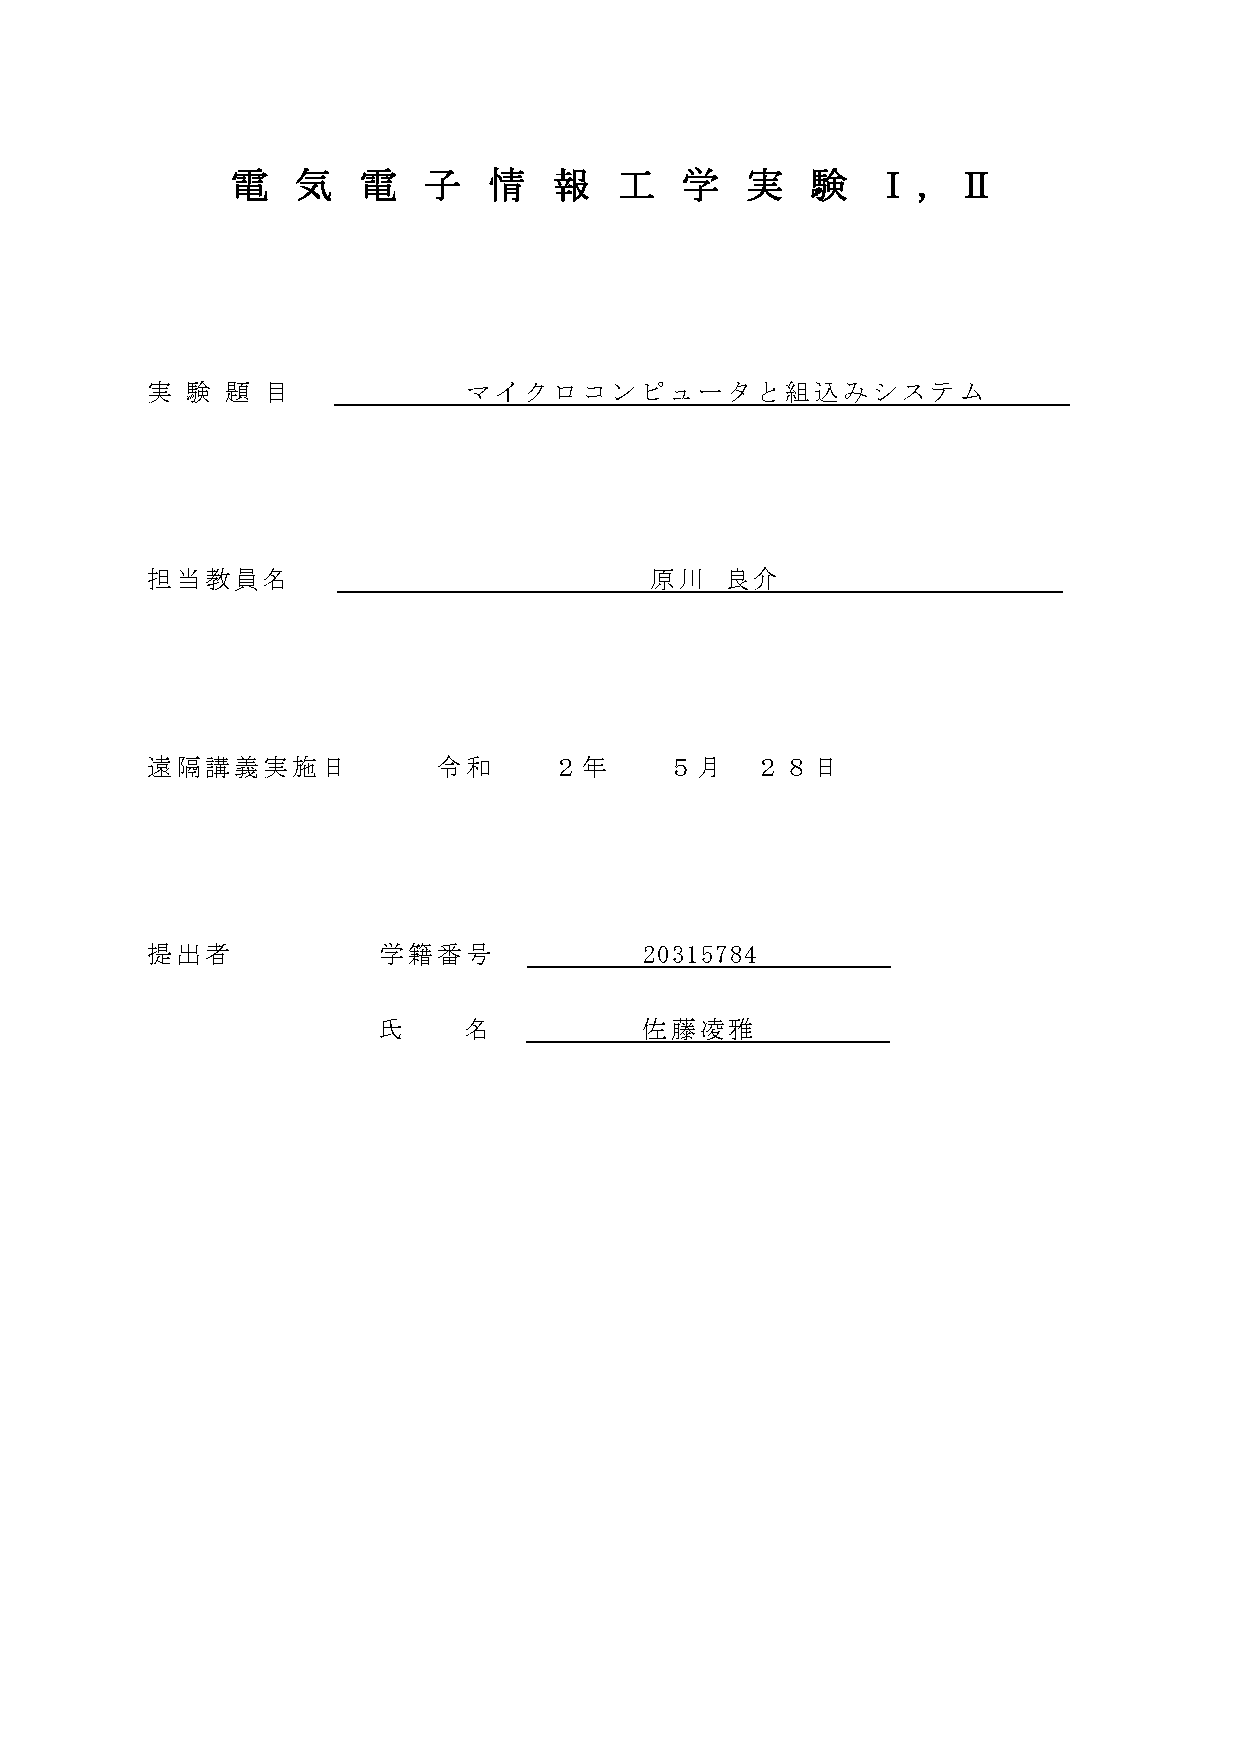
\includepdf[pages=-]{./setting/cover.pdf}
\fontsize{11.041pt}{16.562pt}\selectfont


% 実験の目的,手段,結果,結論を簡潔にまとめ示すこと.(250字程度)
\section{概要 Abstract}
 この実験では与えられた設計仕様を満たすエレベータの組込みシステムの構築を行う.要求された仕様を満たすことのできるプログラムを作成するため,フローチャートを作成し,処理の流れを視覚的にわかりやすい形で記述する.記述されたフローチャートに沿ってアセンブリ言語でのプログラミングを行い,エレベータのシステムを製作する.実験にて作成したシステムの動作を確認する.また,システム構築の過程で組込みシステム設計の動作原理を理解する.


% テキストに書かれている目的等を参考に,各自どの点に注目して実験したのかを明確に示すこと.(300字程度)
\section{目的 Purpose}
 エレベータのシステム開発を通じて組込みシステムの動作原理を理解する.また,システムの構築にはZ80アセンブリ言語によるプログラミングで実装を行う.高級言語のC言語とは異なる機械よりのアセンブリ言語のコーディング能力を体得する.\\
 さらに,グループ作業を通じて,限られた時間での効率的な作業方法などについても検討する.\\
 加えて,与えられた設計仕様を満たすエレベータの組込みシステムの構築を目指し,要求された仕様を満たすことのできるプログラムを作成する.そのために,フローチャートをや仕様書の書き方についても習得する.


% 各自の実験目的に必要な理論的な背景を示すこと.必要ならば,参考文献リストより文献番号を引用すること.(レポート用紙1枚程度)
\section{理論的背景 Theory}
\subsection{Z80マイコン}
 ZiLOGによって開発された8ビットマイクロプロセッサーの一つ.1980年代に広く使われ,パーソナルコンピュータのCPUとしてなど,幅広い用途に使用された.以後も周辺デバイスを集積した製品が出されるなど,現在でも組込み用途において各種機器に使用されている.\cite{z80}

\subsection{アセンブリ言語}
 アセンブリ言語とは,プログラミング言語の類型の一つで,コンピュータのCPU(MPU/マイクロプロセッサ)が直接解釈・実行できる機械語(マシン語)と正確に対応する命令語で構成された言語のことである.\cite{assembly}\\
コード作成の際の注意事項を以下に示す(実験書より引用).
\begin{itemize}
    \item 大文字と小文字、空白(スペース)とタブは同一の文字と認識される.
    \item 複数の連続した空白は一つの空白とみなす.空行は無視される.
    \item ラベル名は6文字以下の英数字、ただし先頭文字は英字.
    \item ラベル名のコロン(:)の直後は空白が必要
    \item コンマ(,)の直後に空白を入れてはいけない.
    \item セミコロン(;)以降はコメントで無視される.
    \item 行送り(インデント)は自由.インデントを揃えなくてもエラーにはならない.
    \item プログラム末尾はEND文(ENDの行も必ず改行する).
\end{itemize}

主な制御命令をTable\ref{table:ControlInstructions}に示す(実験書より引用).
\begin{table}[hbtp]
    \caption{Z80 Assembly Language Main Control Instructions}
    \label{table:ControlInstructions}
    \centering
    \begin{tabular}{lll}
    \hline
    命令名 & 書式 & 内容\\
    \hline \hline
    LD   & A,n    & A ← n\\
    LD   & A,B    & A ← B\\
    ADD  & A,n    & A ← A + n\\
    SUB  & n      & A ← A - n\\
    AND  & s      & A ← (A AND s)\\
    OR   & s      & A ← (A OR s)\\
    SLA  & r      & rレジスタを左へビットシフトする(最下位ビットは0に)\\
    SRL  & r      & rレジスタを右へビットシフトする(最上位ビットは0に)\\
    SET  & n,A    & Aレジスタのnビット目を1にする\\
    BIT  & n,A    & Aレジスタのnビット目の状態をみる\\
    JP   & nn     & nnにジャンプする\\
    JP   & Z, nn  & もし0ならばnnにジャンプする\\
    JP   & NZ,nn  & もし0でなければnnにジャンプする\\
    CALL & nn     & サブルーチンnnにジャンプする\\
    RET  &        & メインルーチンに復帰する\\
    IN   & A,(nn) & nnポートの内容をAレジスタに入れる\\
    OUT  & (nn),A & Aレジスタの内容をnnポートに出力する\\
    \hline
    \end{tabular}
\end{table}


% 実験手段,測定系の概要,測定装置の名称・型番等を書くこと.また,装置の精度・仕様等の情報もできる限り示すこと.(レポート用紙2枚程度)
\section{実験方法 Experiment}
\subsection{実験機器}
 実験にはパソコン,Z80CPU搭載のマイクロコンピュータボード,エレベータ模型を使用する.\\
 エレベータ模型には昇降機,各階乗り場の現在階表示ランプ,エレベータ内の現在階表示ランプ,ドア開閉ボタン,行き先階ボタン,各階乗り場の上下ボタンが備え付けられている.各ボタンにもランプも備え付けられている.

\subsection{課題3}
 1階と2階のみ上下するエレベータの使用設計とフローチャートの作成を行う.

\subsubsection{設計仕様}
\begin{itemize}
    \item エレベータの初期位置がわからない可能性があるので,システム実行時にまずエレベータを1階に持ってくる.
    \item 1階乗り場上ボタン,2階乗り場下ボタンが押された時には押された階にエレベータを持ってくる.
    \item 1階乗り場上ボタン,2階乗り場下ボタンが押された時には押されたボタンのランプを点灯する.
    \item エレベータが到着したら乗り場現在階ランプを点灯する.
    \item 人が乗り込み,行き先階ボタンが押されたら押されたボタンを点灯し,乗り場上下ボタン,現在階ランプを消灯する.そして,移動を開始する.
    \item 人が乗り込まない場合に他の階から呼び出しがあった場合には呼び出された階に持っていく.
    \item エレベータが目的階に到着したら,行き先階ボタンを消灯する.
\end{itemize}

\subsubsection{授業内で作成したフローチャート}
 授業内で作成した課題3のフローチャートをFig.\ref{fig:kadai3_before}に示す.
\begin{figure}[H]
    \centering
    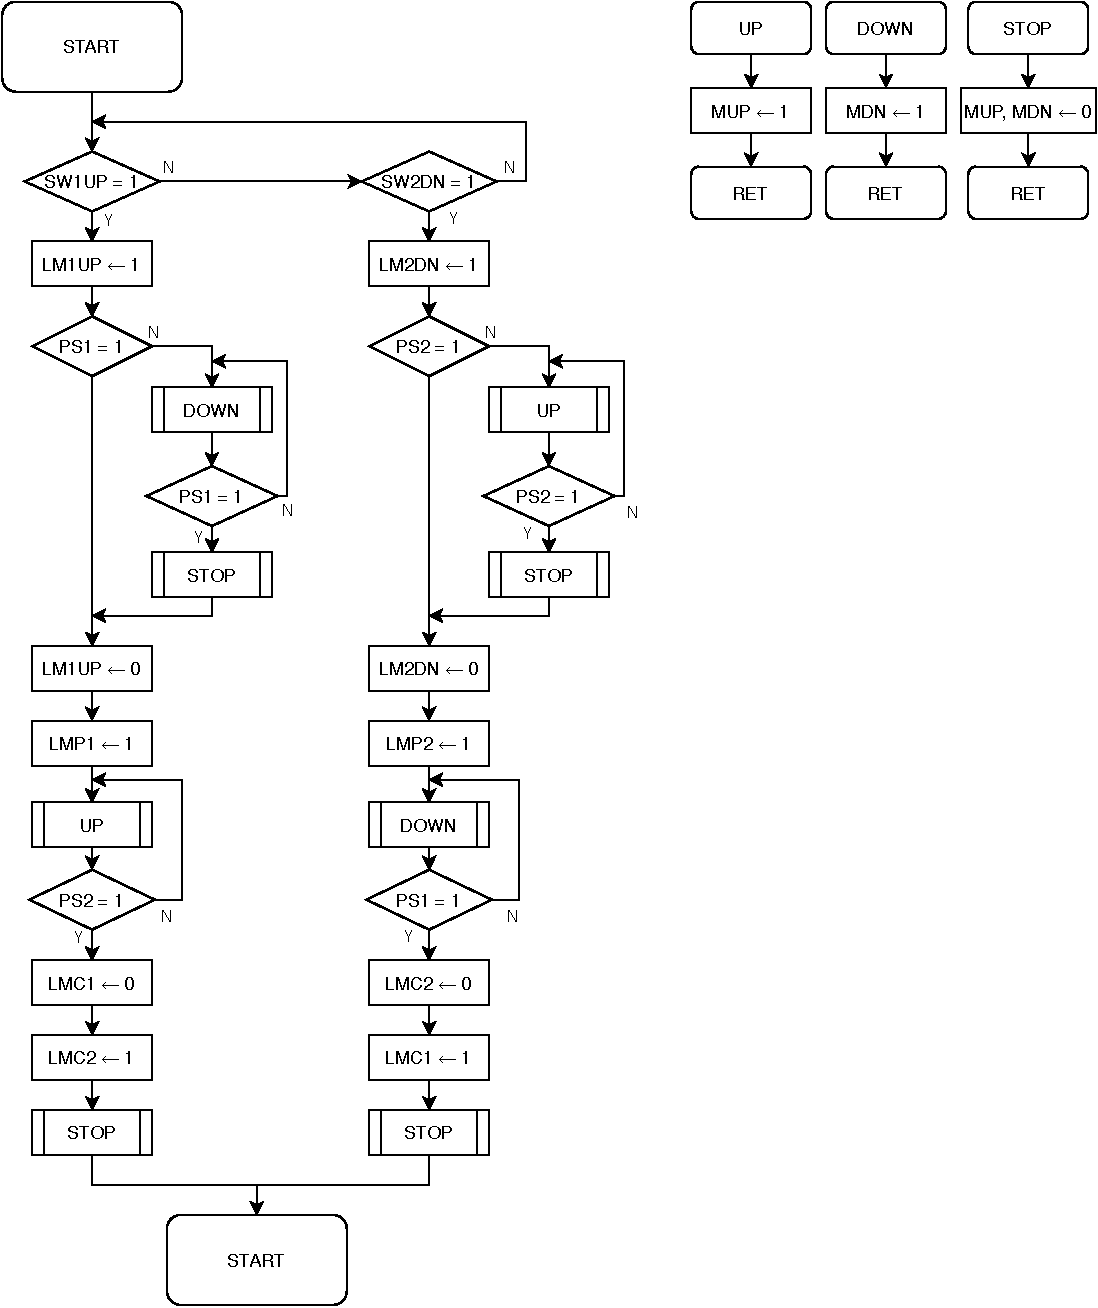
\includegraphics[width=10cm]{./fig/kadai3_before.pdf}
    \caption{Flowchart for homework3 created in class}
    \label{fig:kadai3_before}
\end{figure}

\subsubsection{書き直したしたフローチャート}
 その後,自分で修正したフローチャートをFig.\ref{fig:kadai3}に示す.
\begin{figure}[H]
    \centering
    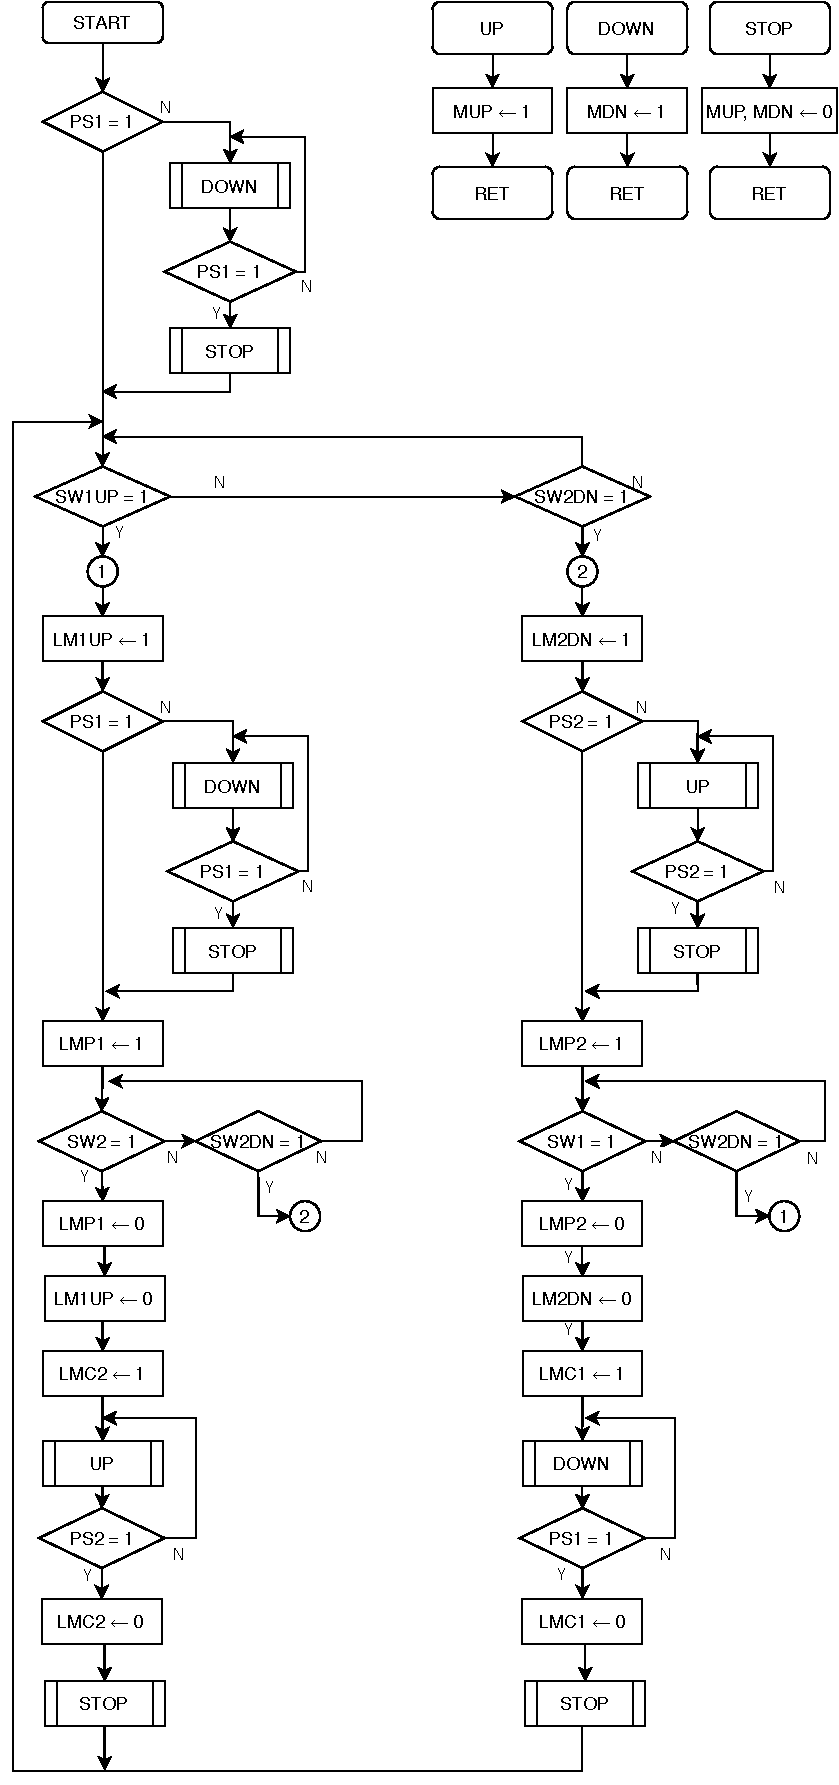
\includegraphics[width=9cm]{./fig/kadai3.pdf}
    \caption{Modified flowchartfor homework3}
    \label{fig:kadai3}
\end{figure}


\subsection{課題4}
 実際の4階エレベータに出来るだけ動作を近づけたエレベータの使用設計とフローチャートの作成を行う.

\subsubsection{設計仕様}
\begin{itemize}
    \item エレベータの初期位置がわからない可能性があるので,システム実行時にまずエレベータを1階に持ってくる.
    \item 各階乗り場上下ボタンが押された時には押された階にエレベータを持ってくる.
    \item 各階乗り場上下ボタンが押された時には押されたボタンのランプを点灯する.
    \item エレベータが到着したら乗り場現在階ランプを点灯する.
    \item 行き先階ボタンが押されたら押されたボタンを点灯する.
    \item 行き先階ボタンが押されたら乗り場上下ボタン,現在階ランプを消灯する.
    \item 行き先階ボタンが押されたら移動を開始する.
    \item 人が乗り込まない場合に他の階から呼び出しがあった場合には呼び出された階に持っていく.
    \item エレベータが目的階に到着したら,行き先階ボタンを消灯する.
\end{itemize}

\subsubsection{授業内で作成したフローチャート}
 授業内で作成した課題3のフローチャートをFig.\ref{fig:kadai4_before}に示す.
\begin{figure}[H]
    \centering
    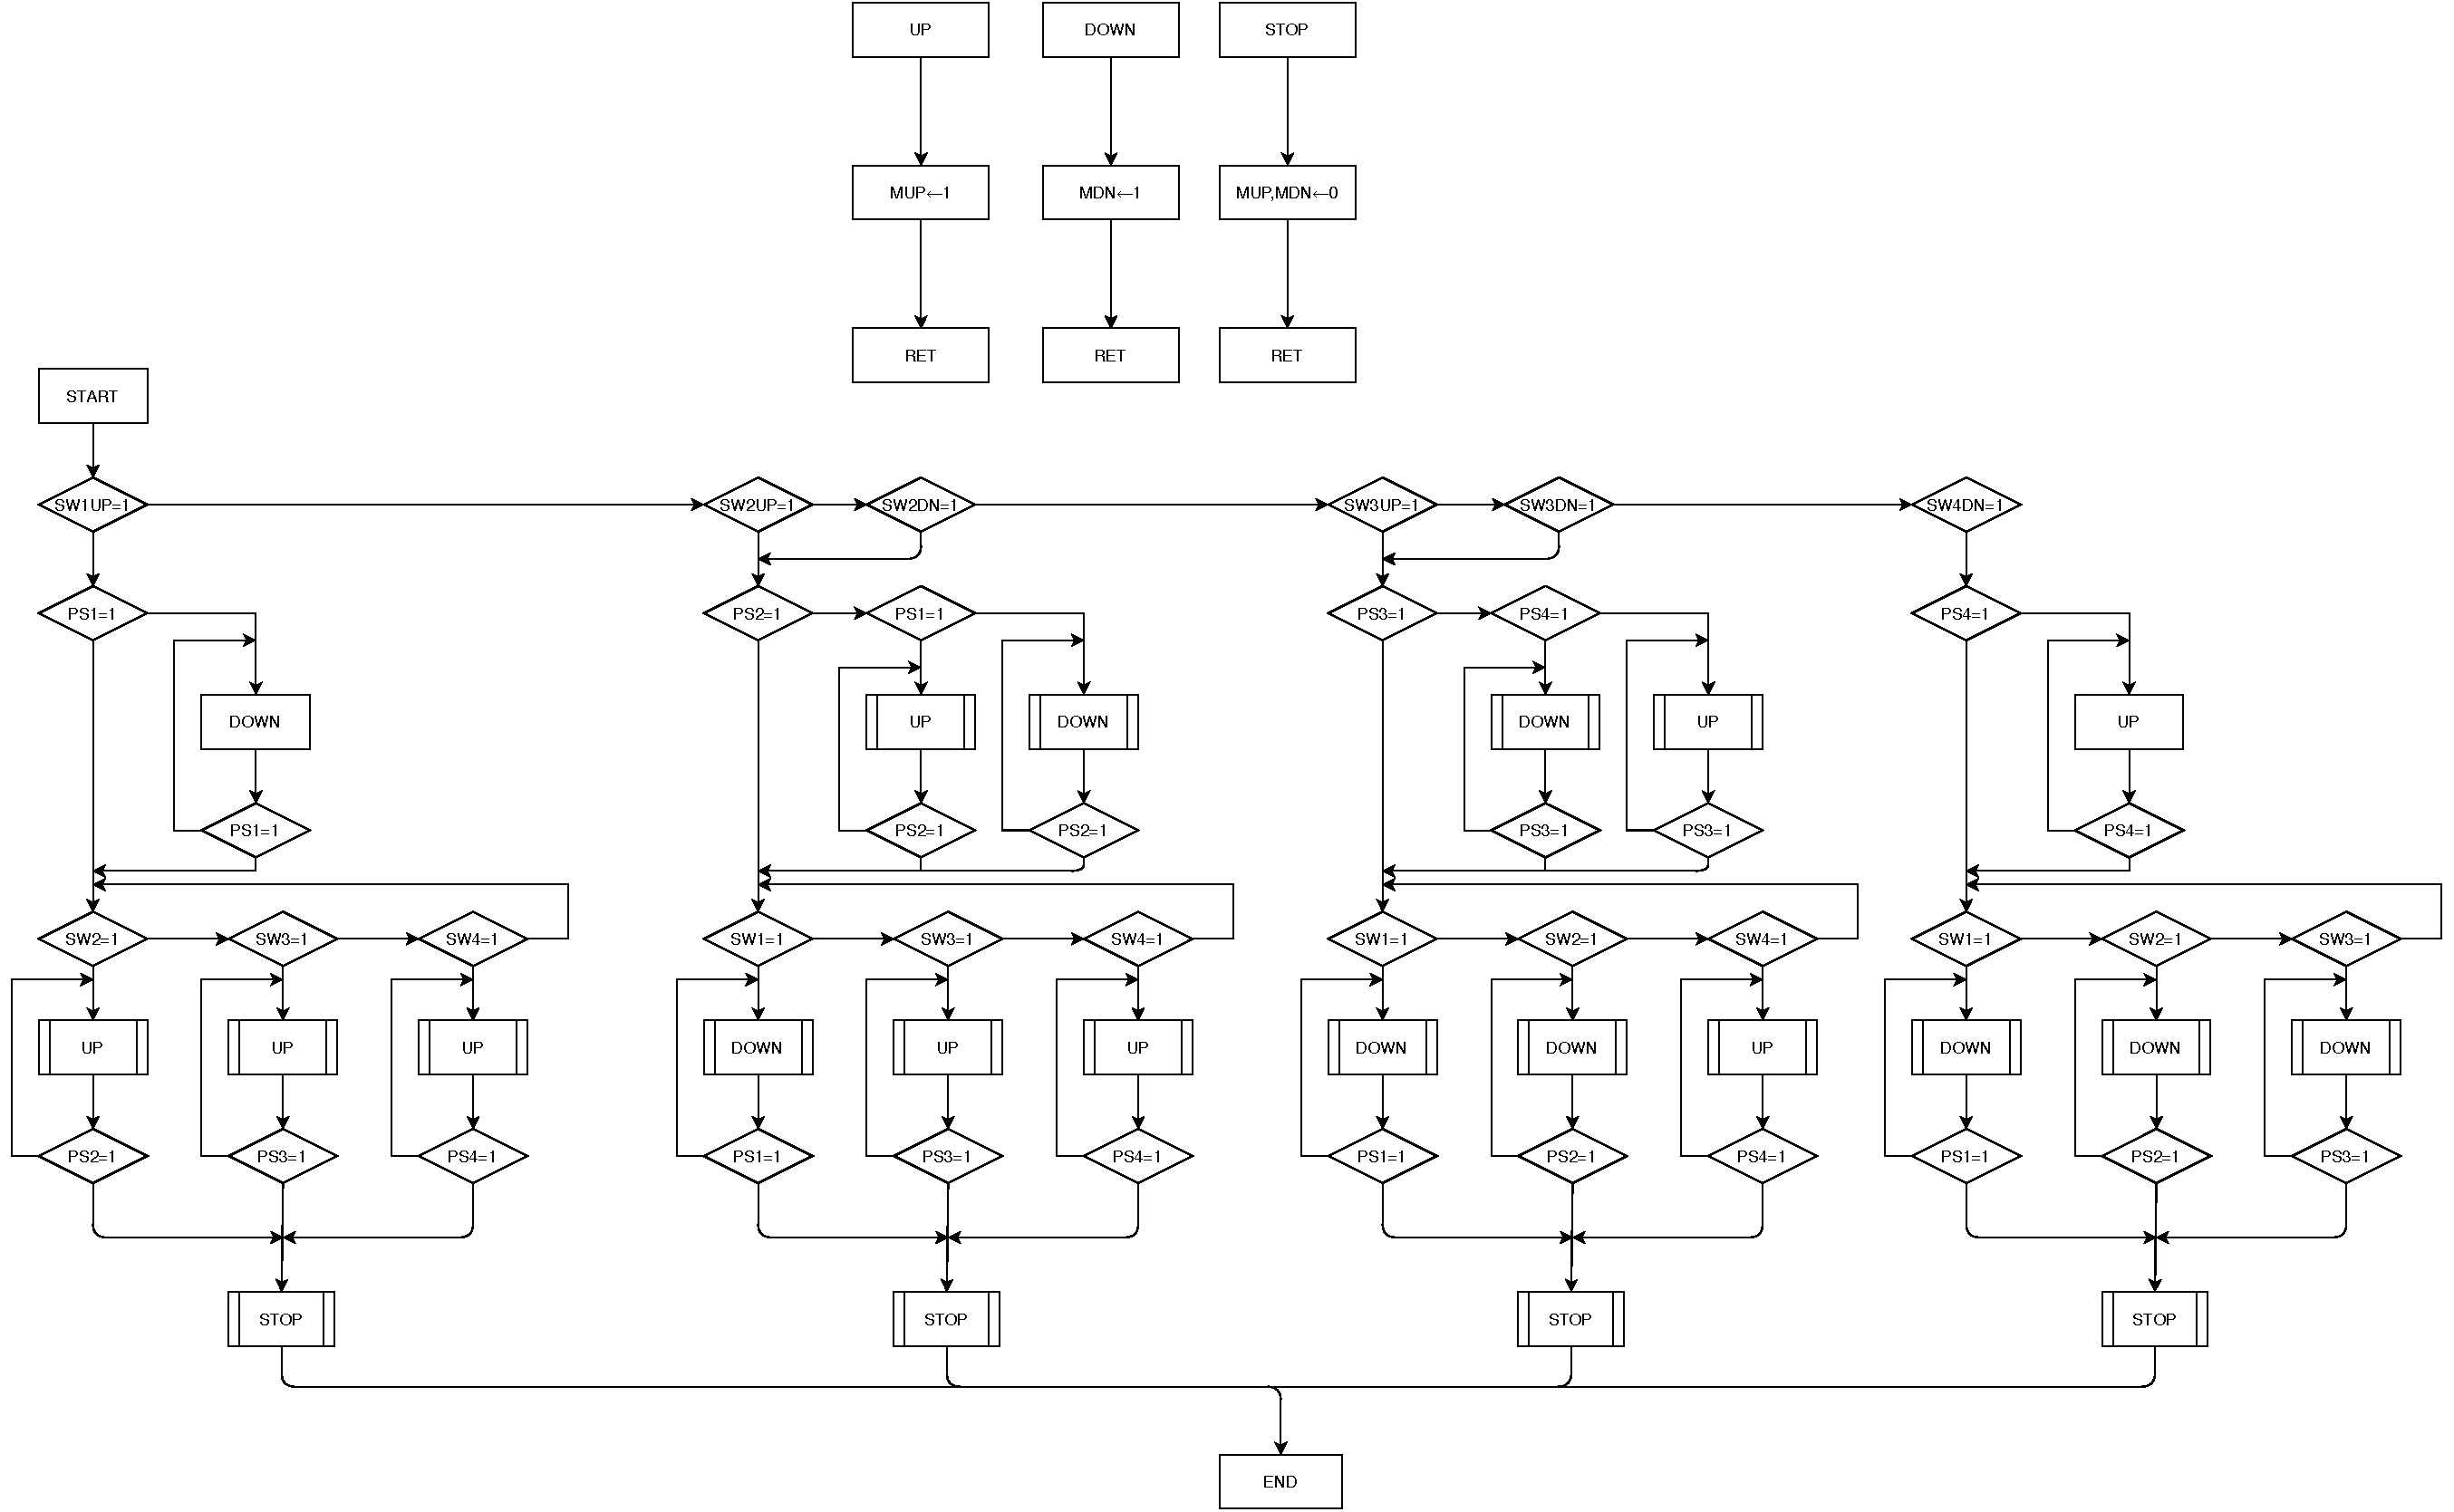
\includegraphics[width=14cm]{./fig/kadai4_before.pdf}
    \caption{Flowchart for homework4 created in class}
    \label{fig:kadai4_before}
\end{figure}

\subsubsection{書き直したしたフローチャート}
 その後,自分で修正したフローチャートをFig.\ref{fig:kadai4}に示す.
\begin{figure}[H]
    \centering
    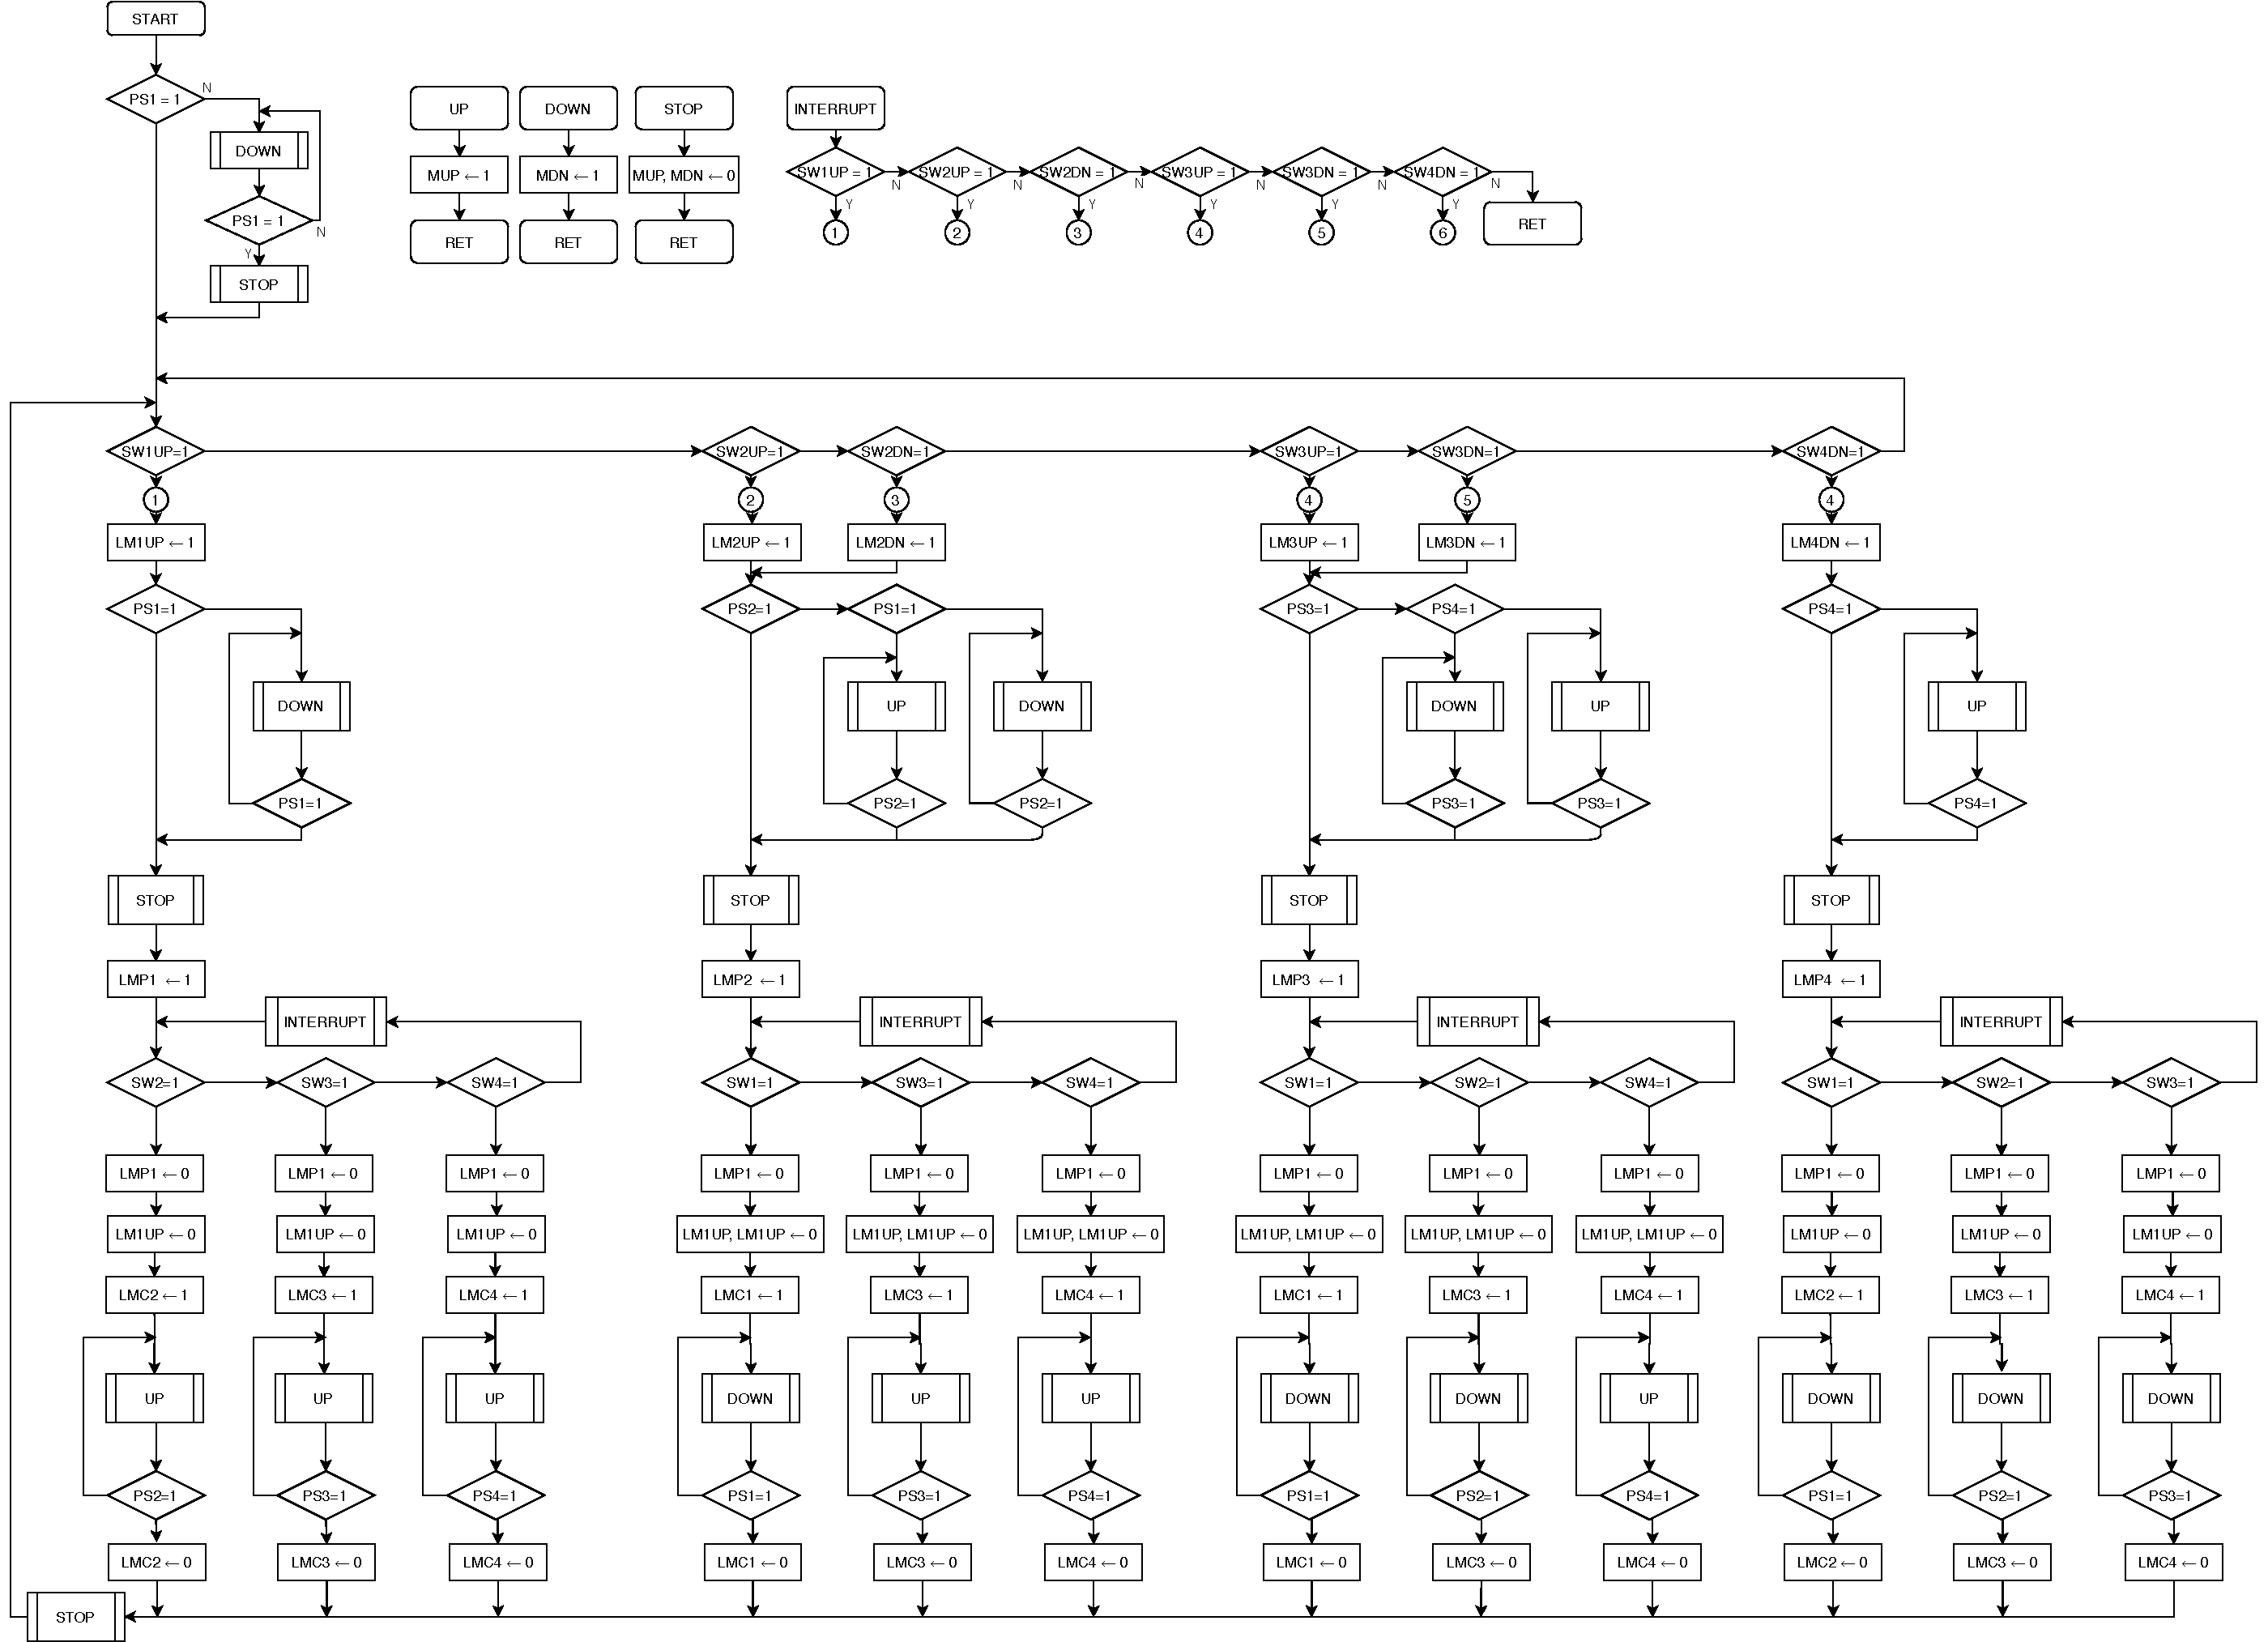
\includegraphics[width=14cm]{./fig/kadai4.pdf}
    \caption{Modified flowchartfor homework4}
    \label{fig:kadai4}
\end{figure}


% % 各自の実験目的に沿った結果を簡潔にまとめること.その他の試行錯誤的実験データは Appendix にまとめる.枚数は各教員の指示に従ってください.(レポート用紙の枚数は教員の指示に従う)
% \section{実験結果 Results}

% % 各自の目的と照らし合わせ,測定結果の妥当性や数値計算結果との整合性などについて考察する.実験結果とサブテキスト/参考書の図式とを比較し議論すること.課題が与えられているテーマに関してはそれについても考察すること.(レポート用紙2枚程度)
% \section{考察 Discussion}

% % 君自身が実験を通じて(実験の方法,まとめ方などで)工夫した点をまとめる.(100字程度 )
% \section{工夫した点}

% 実験結果の羅列ではなく,考察した結果をまとめること.(250字程度)
\section{まとめ Conclusion}
 このレポートでは実験の目的を設定し,Z80マイコンやアセンブリ言語について調査を行った.その後,2通りのエレベータの仕様設計とフローチャートの作成を実施した.2学期の実験では今回作成したフローチャートを元に実際にエレベータの制御システムの構築をし,動作試験を行う.


% レポートで引用した参考文献のリストを付ける.
\section{参考文献 Reference}
\begin{thebibliography}{9}
    \bibitem{z80} 通信用語の基礎知識. Z80. \url{https://www.wdic.org/w/SCI/Z80}, (参照:2020-06-01)
    \bibitem{assembly} IT用語辞典 e-Words. アセンブリ言語とは. \url{https://www.wdic.org/w/SCI/Z80}, (参照:2020-06-01)
\end{thebibliography}


% % 周辺の関連調査事項,作成プログラムリスト,試行錯誤的実験データ
% \appendix
% \section{Appendix}

\end{document}
